\documentclass[11pt,a4paper,twoside]{article}
\usepackage[left=20mm, right=20mm, top=20mm, bottom=20mm]{geometry}
\usepackage{setspace}
\onehalfspacing
\usepackage[T1]{fontenc}
\usepackage[croatian]{babel}

\usepackage[dvipsnames]{xcolor}
\usepackage[most]{tcolorbox}
\definecolor{blue1}{HTML}{DEE3E9}
\definecolor{blue2}{HTML}{F9F9F9}
\definecolor{blue3}{HTML}{9EADC0}

\definecolor{solarized@red}{HTML}{bc658d}
\definecolor{solarized@blue}{HTML}{4677CB}
\definecolor{solarized@green}{HTML}{82c4c3}
\definecolor{solarized@orange}{HTML}{f9d89c}
\definecolor{solarized@background}{HTML}{fbfbfb}

\newenvironment{infoBox}
{
	\begin{tcolorbox}[colback=solarized@background,colframe=solarized@green,enlarge top by=6pt, enlarge bottom by=6pt, title=Informacija]
	}{
	\end{tcolorbox}	
}

\newenvironment{warningBox}
{
	\begin{tcolorbox}[colback=solarized@background,colframe=solarized@orange,enlarge top by=6pt, enlarge bottom by=6pt, title=Upozorenje]
	}{
	\end{tcolorbox}
}

\newenvironment{errorBox}
{
	\begin{tcolorbox}[colback=solarized@background,colframe=solarized@red,enlarge top by=6pt, enlarge bottom by=6pt, title=Mogući problem]
	}{	
	\end{tcolorbox}
}

\newenvironment{comicBox}
{
	\begin{tcolorbox}[colback=solarized@background,colframe=solarized@blue,enlarge top by=6pt, enlarge bottom by=6pt, title=Comic]
	}{	
	\end{tcolorbox}
}

\usepackage{listings}

\lstset
{
	basicstyle=\tiny,
	numbers=left,
	numbersep=5pt,
	numberstyle=\tiny\color{gray},
	showspaces=false,
	tabsize=2,
	columns=fullflexible,
	frame=tb,
	breaklines=true,
	postbreak=\mbox{\textcolor{red}{$\hookrightarrow$}\space},
	xleftmargin=17pt,
	xrightmargin=6pt,
	framexleftmargin=17pt,
	framexrightmargin=5pt,
	framexbottommargin=4pt,
    showstringspaces=false,
}

\lstdefinelanguage{XML}
{
	morestring=[b]",
	morestring=[s]{>}{<},
	morecomment=[s]{<?}{?>},
	stringstyle=\color{black},
	identifierstyle=\color{black},
	keywordstyle=\color{cyan},
	morekeywords={xmlns,version,type,ma-id}% list your attributes here
}

\lstdefinelanguage{Kotlin}
{
	comment=[l]{//},
	commentstyle={\color{gray}\ttfamily},
	emph={filter, first, firstOrNull, forEach, lazy, map, mapNotNull, println},
	emphstyle={\color{OrangeRed}},
	identifierstyle=\color{black},
	keywords={!in, !is, abstract, actual, annotation, as, as?, break, by, catch, class, companion, const, constructor, continue, crossinline, data, delegate, do, dynamic, else, enum, expect, external, false, field, file, final, finally, for, fun, get, if, import, in, infix, init, inline, inner, interface, internal, is, lateinit, noinline, null, object, open, operator, out, override, package, param, private, property, protected, public, receiveris, reified, return, return@, sealed, set, setparam, super, suspend, tailrec, this, throw, true, try, typealias, typeof, val, var, vararg, when, where, while},
	keywordstyle={\color{NavyBlue}\bfseries},
	morecomment=[s]{/*}{*/},
	morestring=[b]",
	morestring=[s]{"""*}{*"""},
	ndkeywords={@Deprecated, @JvmField, @JvmName, @JvmOverloads, @JvmStatic, @JvmSynthetic, Array, Byte, Double, Float, Int, Integer, Iterable, Long, Runnable, Short, String, Any, Unit, Nothing},
	ndkeywordstyle={\color{BurntOrange}\bfseries},
	sensitive=true,
	stringstyle={\color{ForestGreen}\ttfamily},
} 

% Handling figures:
\usepackage{graphicx}
\graphicspath{{../figures/}}

\begin{document}
	
\section{Uvod}

	Razvoj mobilnih aplikacija jedna je od radionica u sklopu projekta Studentsko poduzetništvo - 404 koji se izvodi 2023. u suradnji Fakulteta elektrotehnike, računarstva i informacijskih tehnologija Osijek (FERIT), Fakulteta primijenjene matematike i informatike u Osijeku (MATHOS) te Ekonomskog fakulteta u Osijeku (EFOS). Cilj radionice jest pokazati učenicima osnovne koncepte razvoja mobilnih aplikacija s fokusom na platformu Android te ih potaknuti na samostalno učenje i istraživanje.
	
	Ovaj minijaturni priručnik prati aktivnosti radionice gdje će se kroz kreiranje nove Android aplikacije učenici upoznati s osnovnim pojmovima kao što su izgradnja korisničkog sučelja, povezivanje programskog koda i elemenata korisničkog sučelja, ali i sa složenijim elementima aplikacija poput uporabe senzora ili prikaza podataka dostupnih na Internetu. Aplikacija koja će biti izrađena sastoji se od tri zasebna ekrana, ekrana za inspiraciju koji će poslužiti za prolazak kroz osnove kreiranja korisničkog sučelja, ekrana za igru koji će poslužiti za upoznavanje sa senzorima te ekrana za šalu koji će poslužiti za dohvaćanje podataka s interneta i njihov prikaz. Svijet razvoja mobilnih aplikacija puno je širi od sadržaja koji pokriva radionica pa će u posljednjem poglavlju biti prikazane poveznice na vanjske resurse koje je moguće koristiti za samostalan rad i učenje. Za sve naknadne informacije i pitanja, slobodno se javite putem e-maila na bruno.zoric@ferit.hr.
	
	\begin{infoBox}		
		
	\end{infoBox}
	
\section{Instalacija alata}

\begin{figure}[!h]
	\centering
	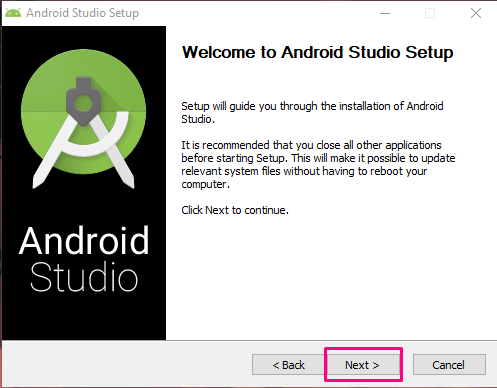
\includegraphics{install_01.png}
	\caption{Instalacija Android Studija - 1. korak}
	\label{fig:install_01}	
\end{figure}

\begin{figure}[!h]
	\centering
	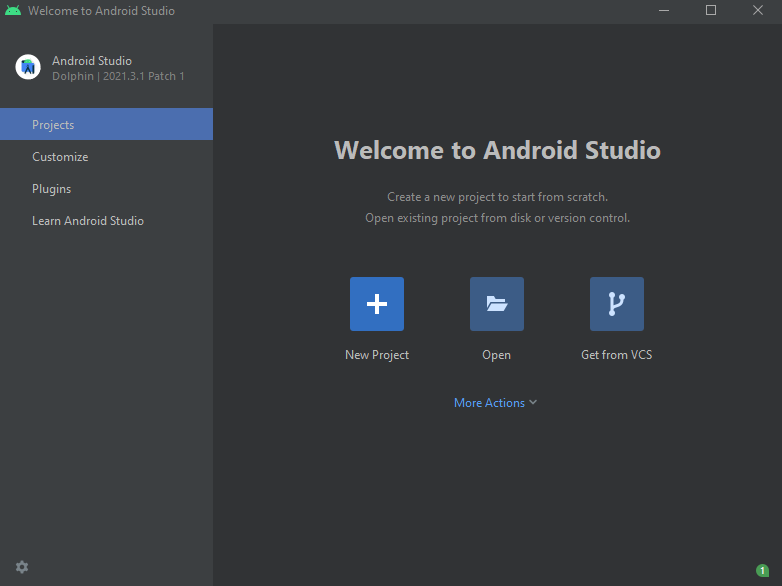
\includegraphics[width=\textwidth]{install_02.png}
	\caption{Instalacija Android Studija - 2. korak}
	\label{fig:install_02}	
\end{figure}

\begin{figure}[!h]
	\centering
	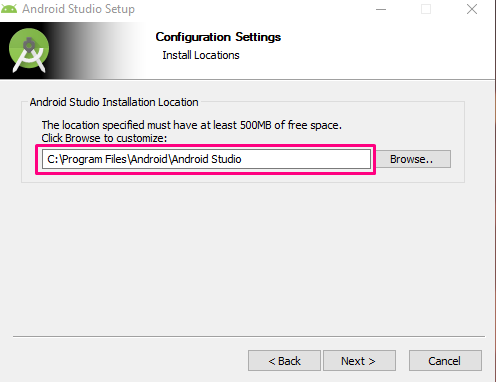
\includegraphics{install_03.png}
	\caption{Instalacija Android Studija - 3. korak}
	\label{fig:install_03}	
\end{figure}

\begin{figure}[!h]
	\centering
	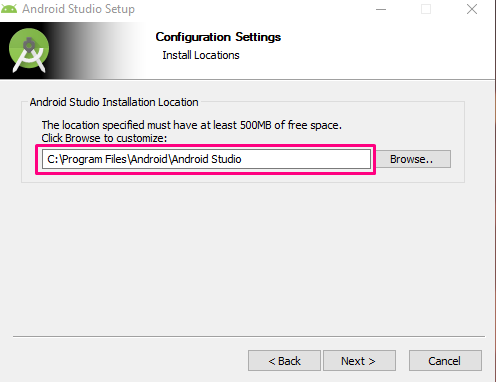
\includegraphics{install_04.png}
	\caption{Instalacija Android Studija - 3. korak}
	\label{fig:install_03}	
\end{figure}

\begin{figure}[!h]
	\centering
	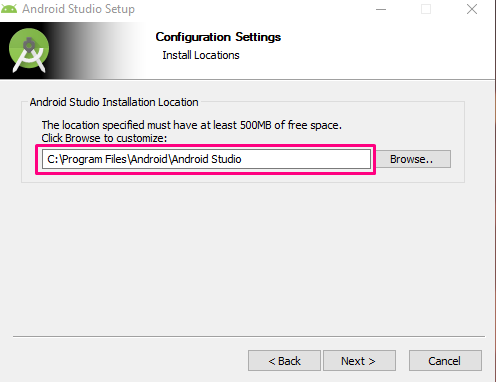
\includegraphics{install_04.png}
	\caption{Instalacija Android Studija - 4. korak}
	\label{fig:install_04}	
\end{figure}

\begin{figure}[!h]
	\centering
	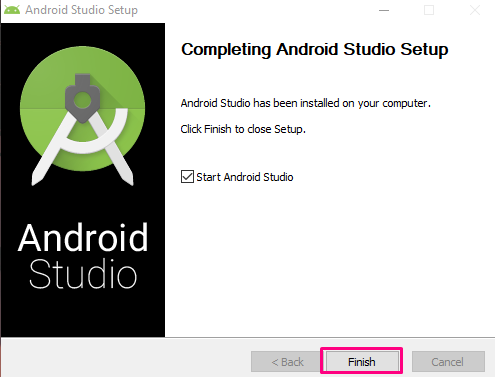
\includegraphics{install_05.png}
	\caption{Instalacija Android Studija - 5. korak}
	\label{fig:install_05}	
\end{figure}

\begin{figure}[!h]
	\centering
	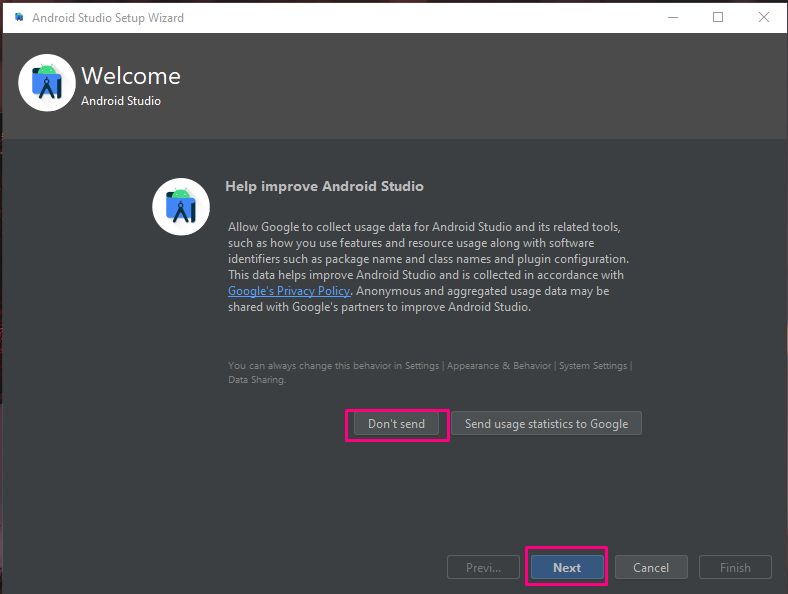
\includegraphics{install_06.png}
	\caption{Instalacija Android Studija - 6. korak}
	\label{fig:install_06}	
\end{figure}

\begin{figure}[!h]
	\centering
	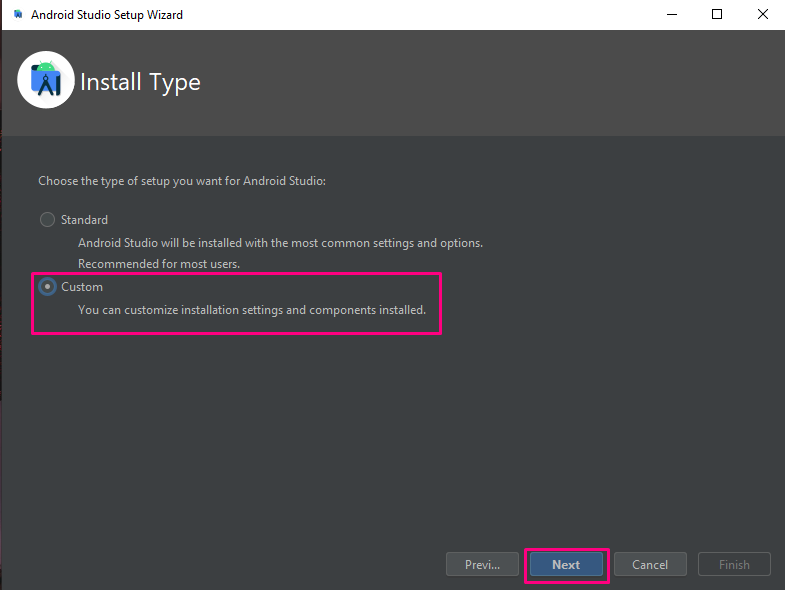
\includegraphics[width=\textwidth]{install_07.png}
	\caption{Instalacija Android Studija - 7. korak}
	\label{fig:install_07}	
\end{figure}

\begin{figure}[!h]
	\centering
	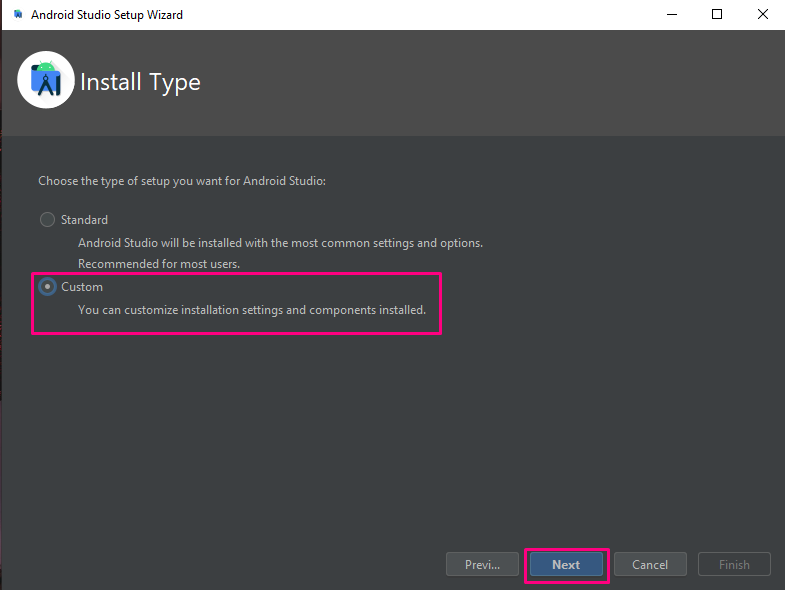
\includegraphics[width=\textwidth]{install_08.png}
	\caption{Instalacija Android Studija - 8. korak}
	\label{fig:install_08}	
\end{figure}

\begin{figure}[!h]
	\centering
	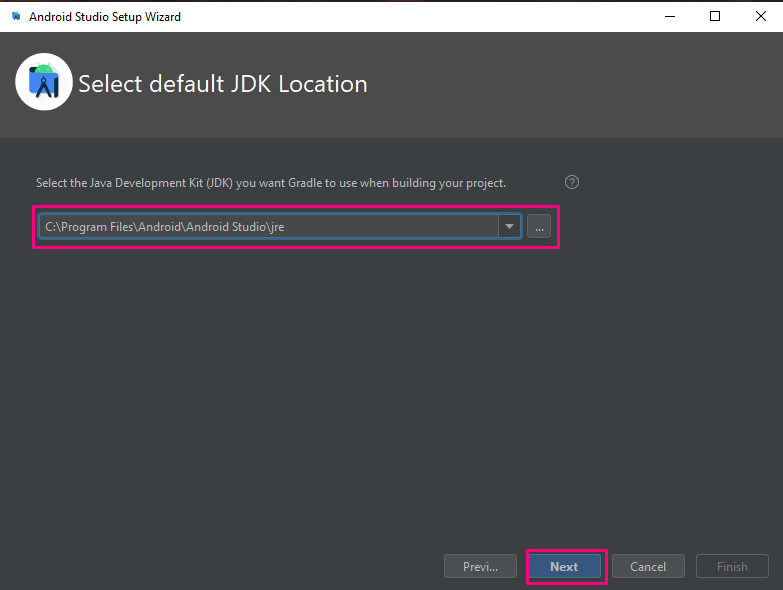
\includegraphics[width=\textwidth]{install_09.png}
	\caption{Instalacija Android Studija - 9. korak}
	\label{fig:install_09}	
\end{figure}

\begin{figure}[!h]
	\centering
	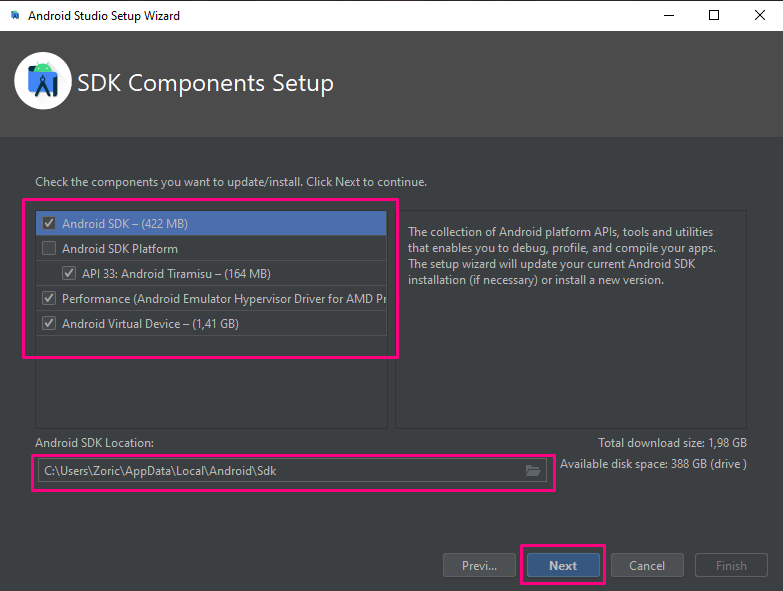
\includegraphics[width=\textwidth]{install_10.png}
	\caption{Instalacija Android Studija - 10. korak}
	\label{fig:install_10}	
\end{figure}

\begin{figure}[!h]
	\centering
	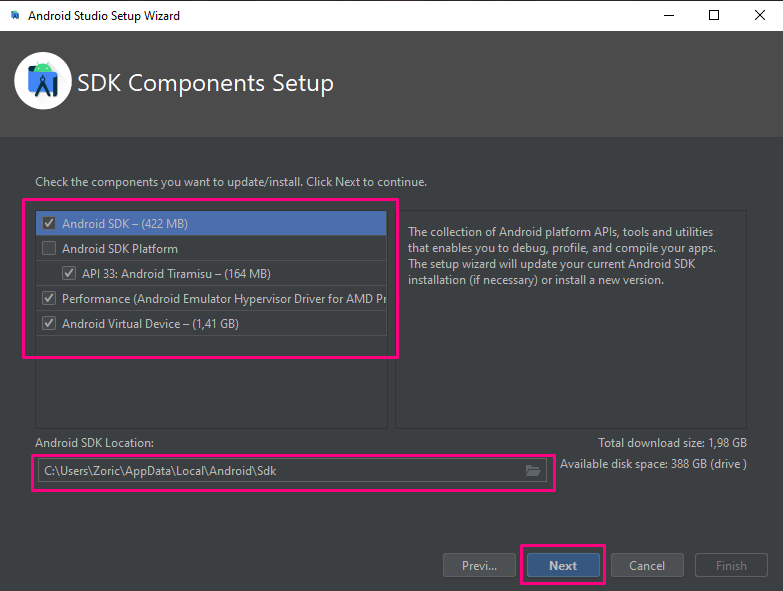
\includegraphics[width=\textwidth]{install_11.png}
	\caption{Instalacija Android Studija - 11. korak}
	\label{fig:install_11}	
\end{figure}

\begin{figure}[!h]
	\centering
	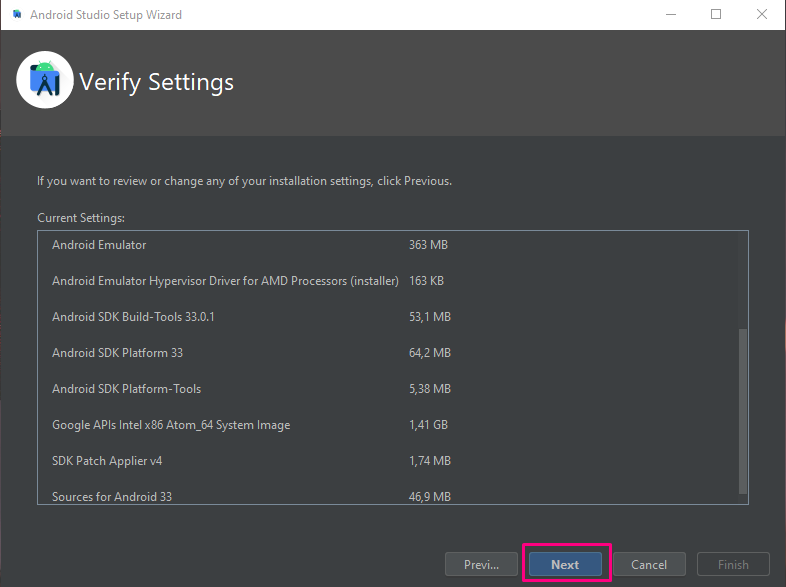
\includegraphics[width=\textwidth]{install_12.png}
	\caption{Instalacija Android Studija - 12. korak}
	\label{fig:install_12}	
\end{figure}

\begin{figure}[!h]
	\centering
	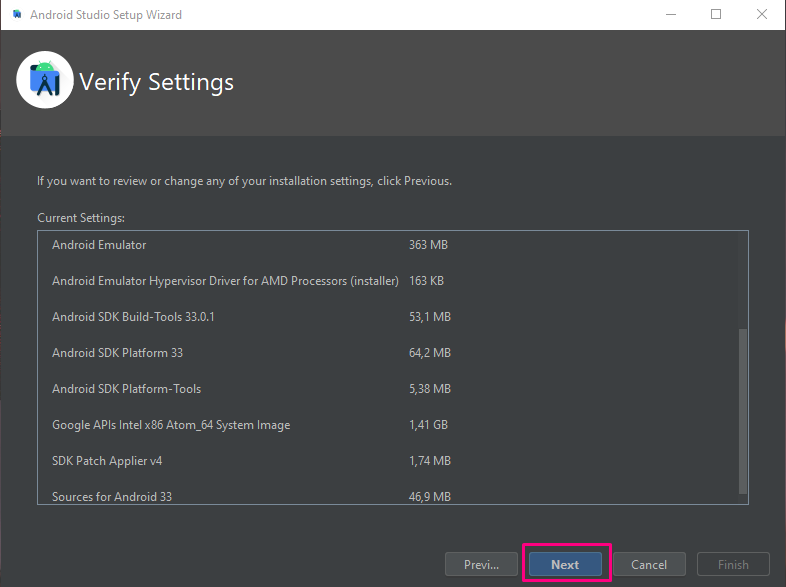
\includegraphics[width=\textwidth]{install_13.png}
	\caption{Instalacija Android Studija - 13. korak}
	\label{fig:install_13}	
\end{figure}

\begin{figure}[!h]
	\centering
	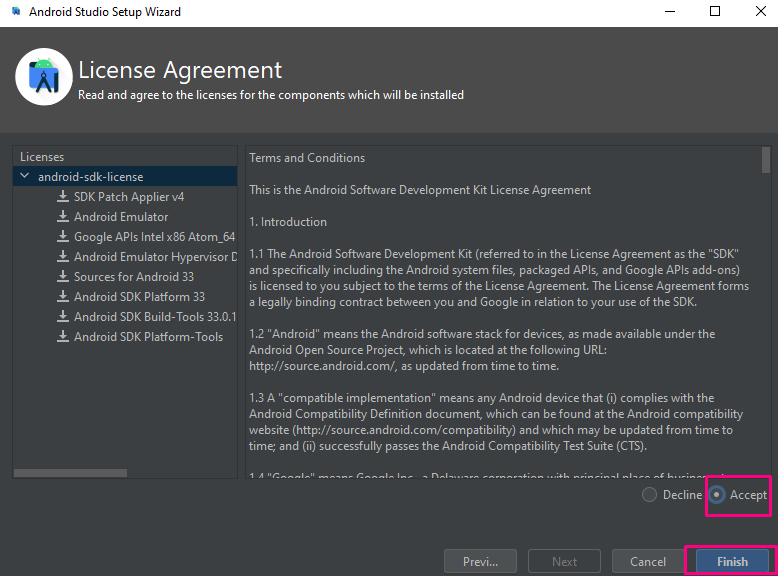
\includegraphics[width=\textwidth]{install_14.png}
	\caption{Instalacija Android Studija - 14. korak}
	\label{fig:install_14}	
\end{figure}

\begin{figure}[!h]
	\centering
	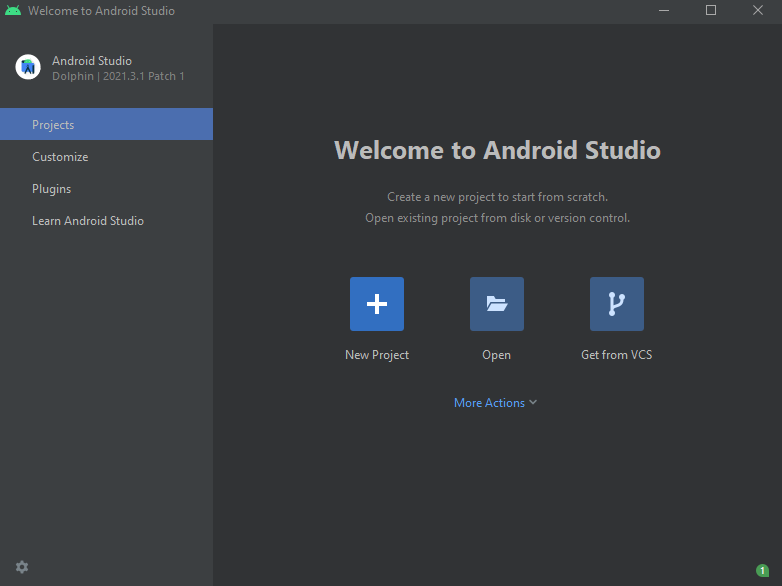
\includegraphics[width=\textwidth]{install_15.png}
	\caption{Instalacija Android Studija - 15. korak}
	\label{fig:install_15}	
\end{figure}

\section{Kreiranje projekta}

\begin{figure}[!h]
	\centering
	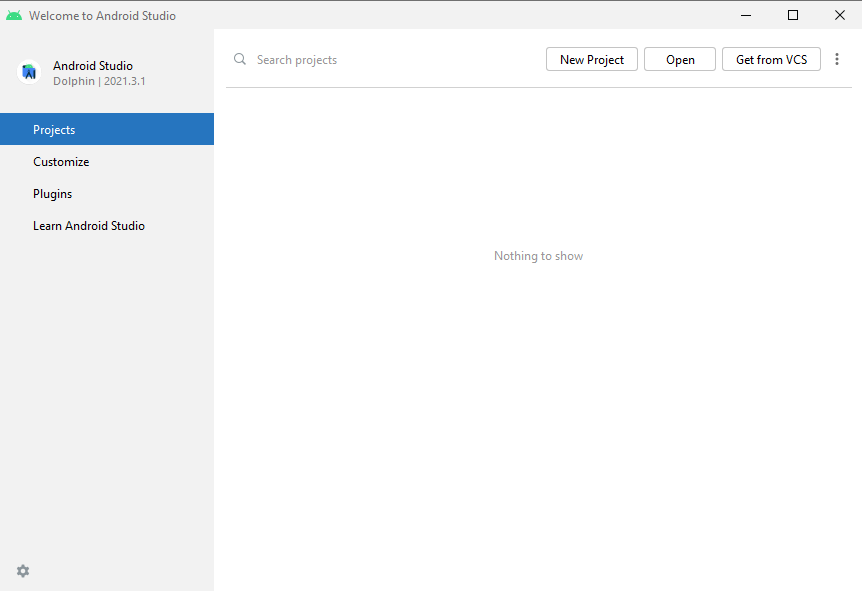
\includegraphics[width=\textwidth]{new_project_01.png}
	\caption{Kreiranje novog projekta - 1. korak}
	\label{fig:new_project_01}	
\end{figure}

\begin{figure}[!h]
	\centering
	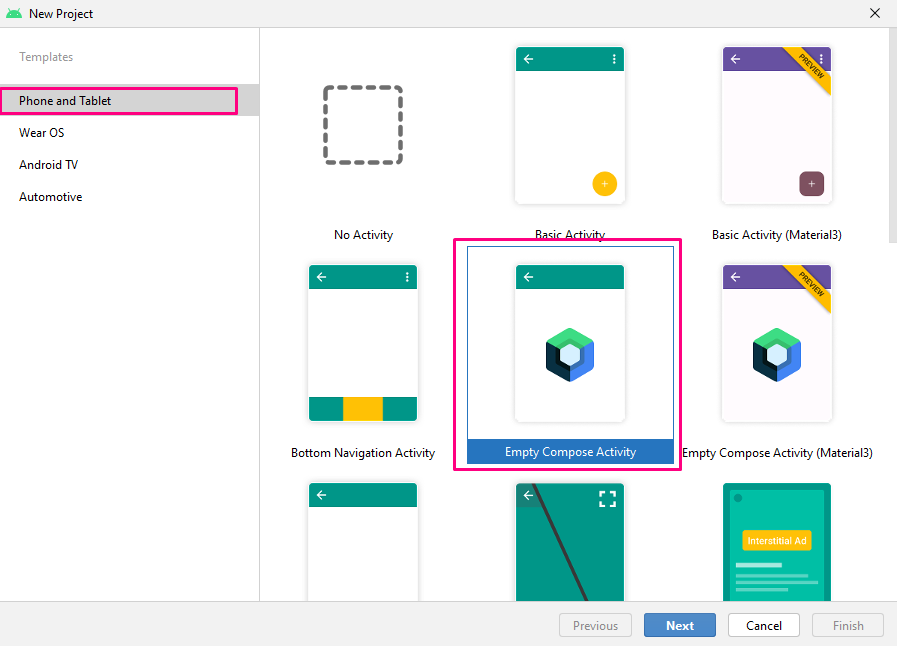
\includegraphics[width=\textwidth]{new_project_02.png}
	\caption{Kreiranje novog projekta - 2. korak}
	\label{fig:new_project_02}	
\end{figure}

\begin{figure}[!h]
	\centering
	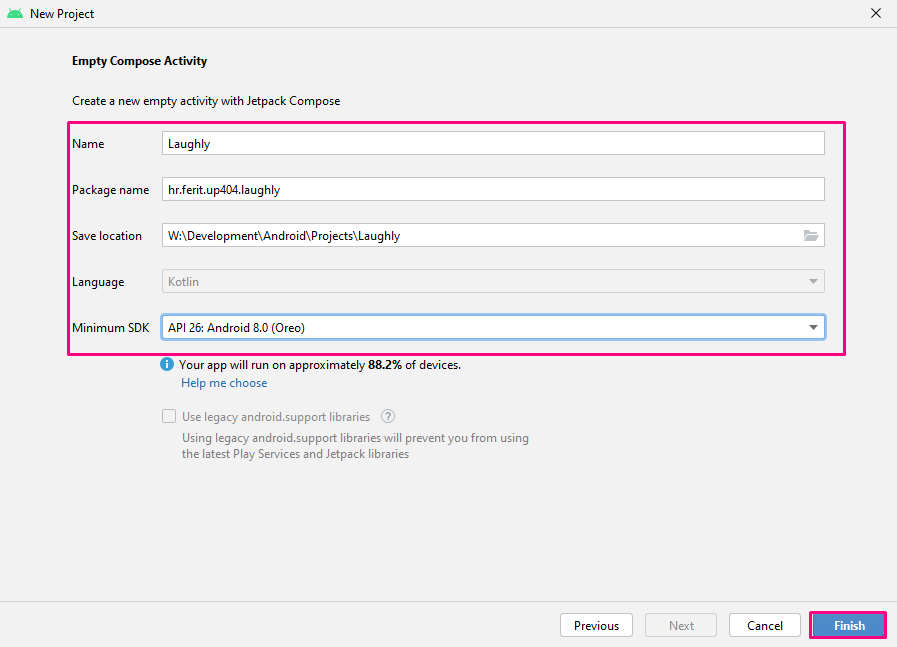
\includegraphics[width=\textwidth]{new_project_03.png}
	\caption{Kreiranje novog projekta - 3. korak}
	\label{fig:new_project_03}	
\end{figure}

\begin{figure}[!h]
	\centering
	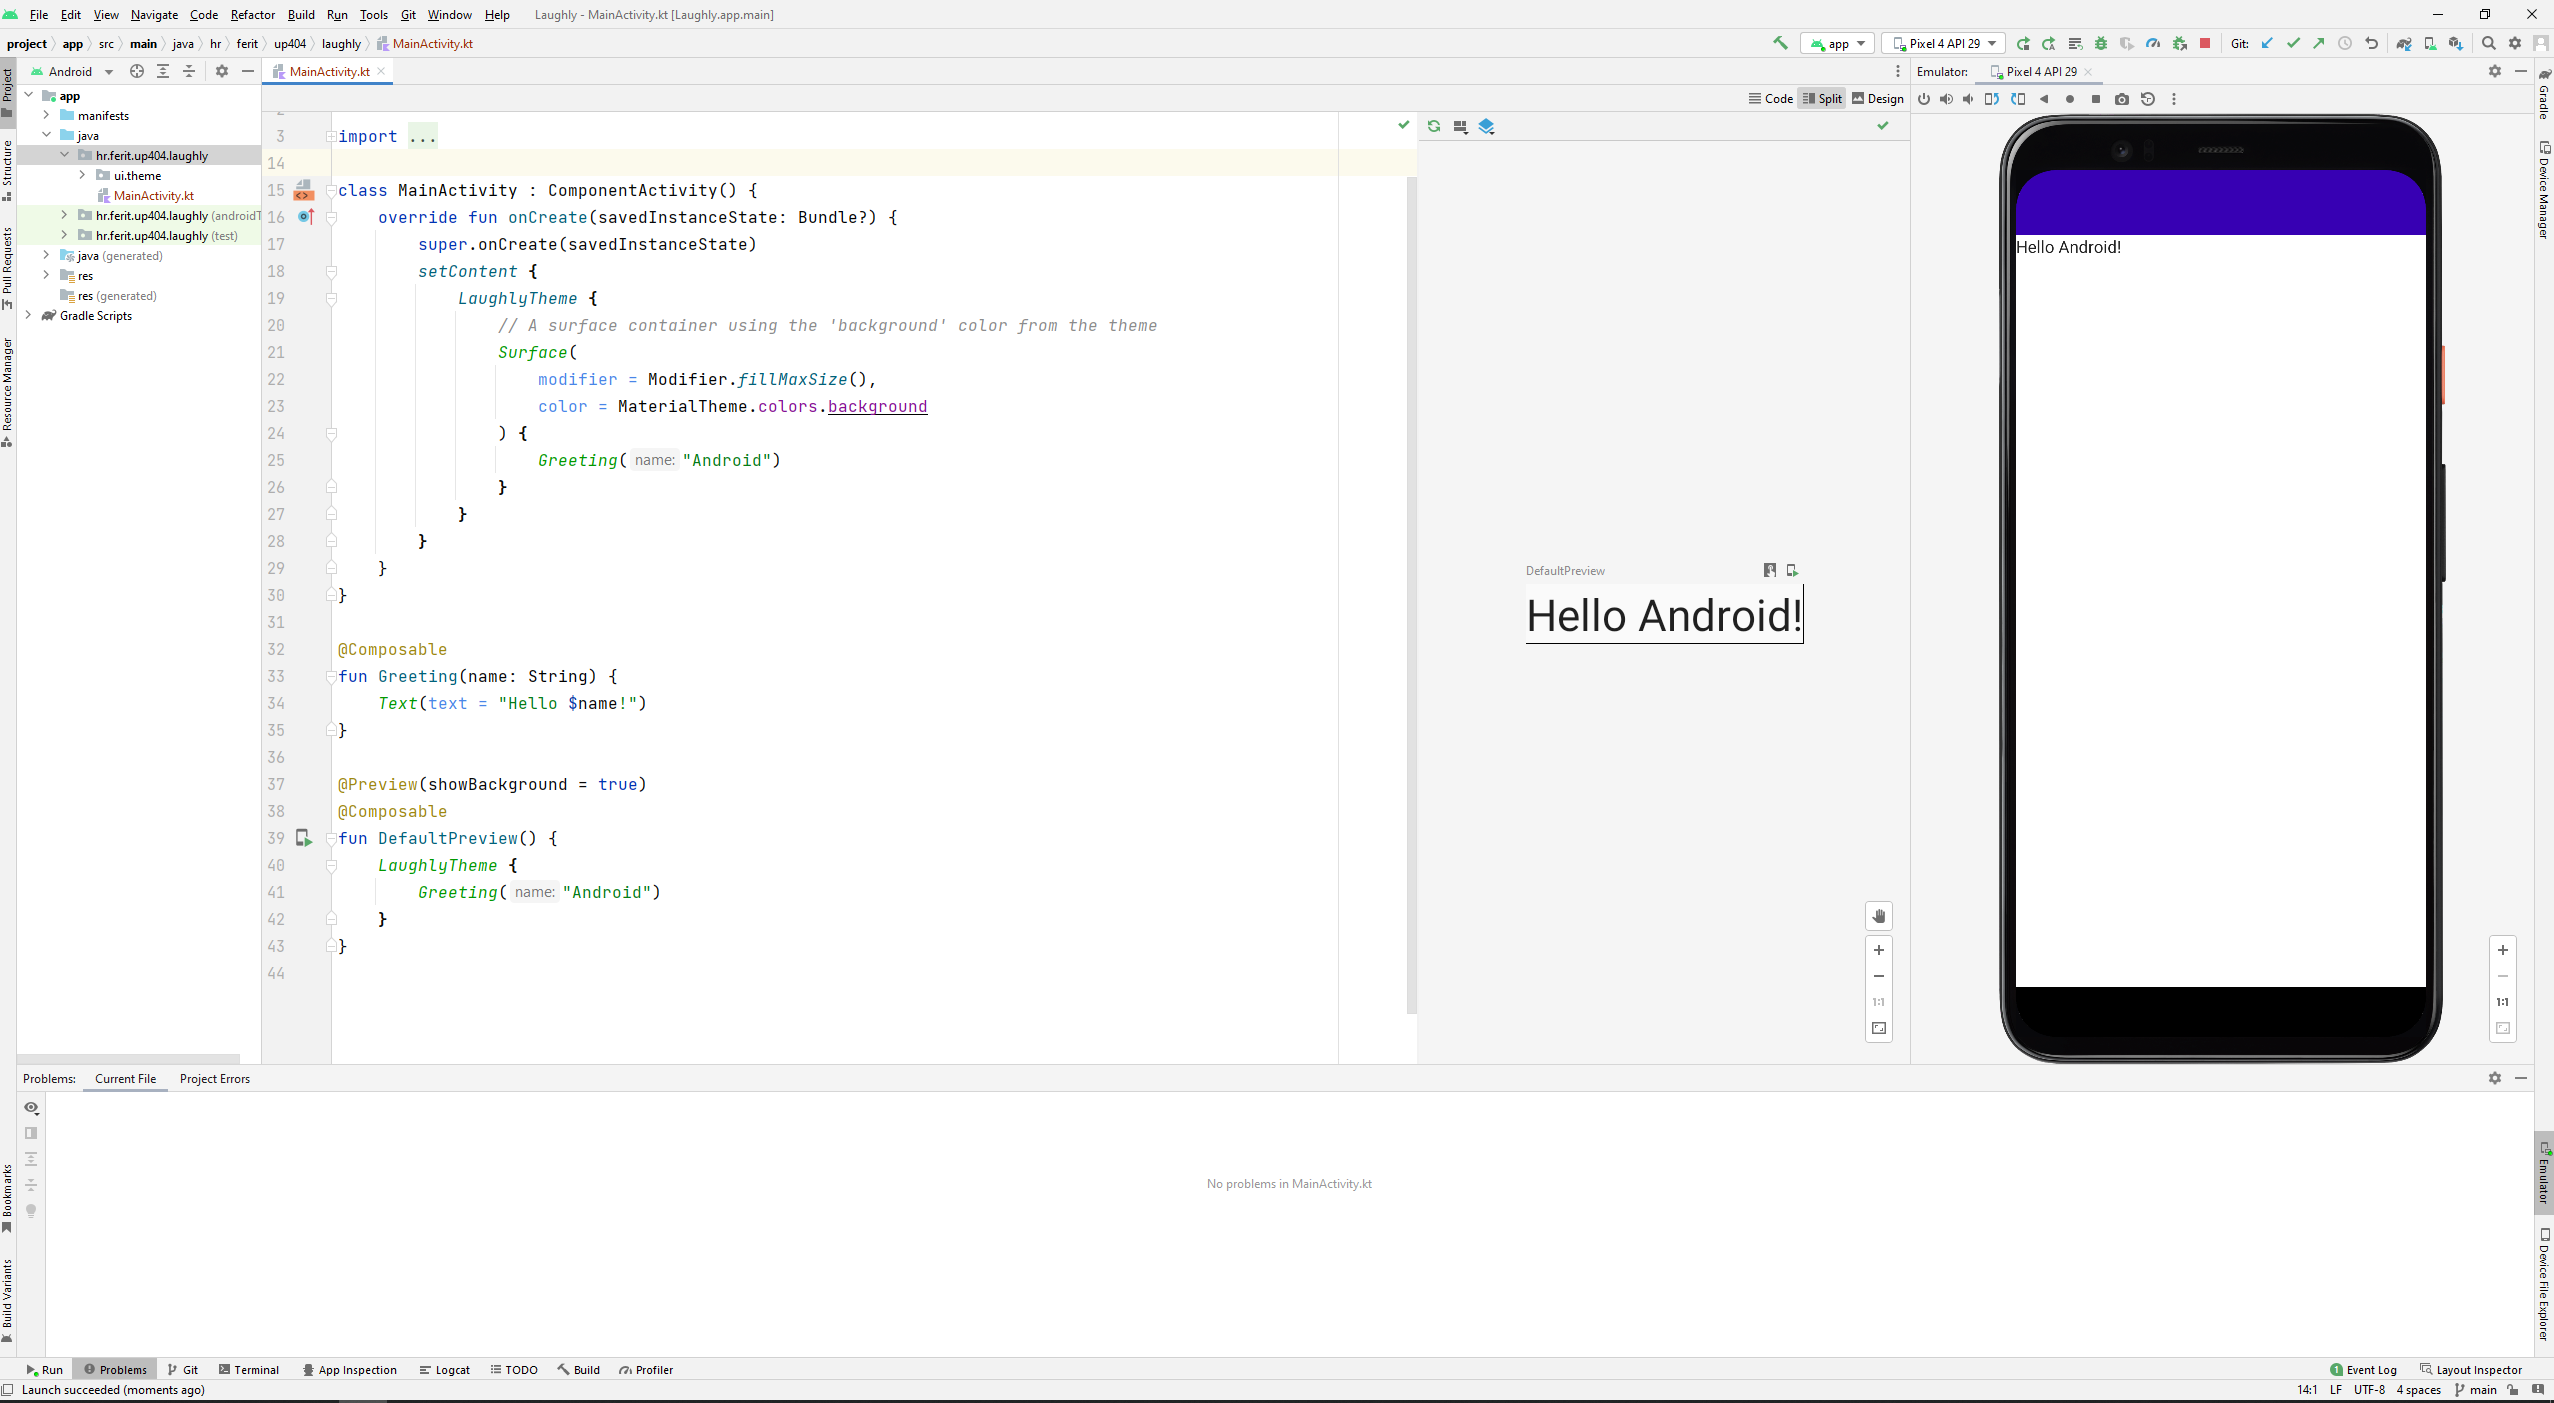
\includegraphics[width=\textwidth]{new_project_04.png}
	\caption{Kreiranje novog projekta - 4. korak}
	\label{fig:new_project_04}	
\end{figure}

\section{Uvođenje ekrana i navigacija}

Android aplikacije u pravilu imaju ekrane koji služe za prikaz sadržaja korisniku. Za potrebe prikaza pojedinog ekrana moguće je koristiti rarzličite gotove komponente koje se zovu \texttt{Activity} ili \texttt{Fragment}. Iako je ranije primaran način za oblikovanje i izgradnju korisničkih sučelja bio napisati \texttt{XML} kod koji ih opisuje i koji se vezuje uz pojedini \texttt{Activity} ili \texttt{Fragment}, danas to više nije tako. U novije vrijeme koristi se pristup gdje je svaka komponenta sučelja, uključujući i cijele ekrane, predstavljena funkcijom. Ovo je omogućeno korištenjem biblioteke imena \texttt{Jetpack Compose}, a taj pristup i navedena biblioteka bit će korišteni i u sklopu ove radionice. U ovom slučaju, mora postojati samo jedan \texttt{Activity} koji će služiti kao polazna točka i kontejner za sve ekrane aplikacije. Sama aplikacija imat će pet ekrana. Glavni ekran (\texttt{MainScreen}) sadržavat će komponente za navigaciju i određivati koji je početni ekran aplikacije. Početni ekran (\texttt{HomeScreen}) sadržavat će gumbe za navigaciju prema pojedinim aktivnostima aplikacije. Tri ekrana koja predstavljaju aktivnosti u aplikaciji bit će redom inspirirajući ekran (\texttt{InspireScreen}), zaigrani ekran (\texttt{PlayScreen}) te nasmijani ekran (\texttt{LaughScreen}). 

Prvi korak koji ćemo napraviti je priprema projekta. Prilikom izrade aplikacije za bilo koju platformu programer se oslanja na kod i alate koje su razvili drugi programeri prije njega, a koji dolaze u obliku pripremljenih biblioteka. S obzirom da ih je razvio netko "izvana", često se nazivaju vanjskim ovisnostima (engl. \textit{external dependency}). U suprotnom bi izrada bila osjetno dugotrajnija i zamornija. Kod Android aplikacija, ove se vanjske ovisnosti uključuju u projekt dodavanjem nekoliko linija koda u datoteku \texttt{build.gradle (Module: app)} gdje se opisuje što točno želimo uključiti i koristiti u našem projektu. Sve potrebne vanjske ovisnosti za cjelokupnu radionicu dane su izlistanjem \ref{lst:dependencies}.

\begin{lstlisting}[caption={Ovisnosnosti o vanjskim bibliotekama u datoteci build.gradle (Module:app)}, label={lst:dependencies}, language=Kotlin]
/***********************************************************************/
/*  Specific dependencies for the workshop:*/
/***********************************************************************/
// Navigation with jetpack compose:
def nav_version = "2.5.3"
implementation "androidx.navigation:navigation-compose:$nav_version"

// Ktor for networking:
def ktor_version = '2.2.2'
implementation "io.ktor:ktor-client-core:$ktor_version"
implementation("io.ktor:ktor-client-android:$ktor_version")
implementation "io.ktor:ktor-client-serialization:$ktor_version"
implementation "io.ktor:ktor-serialization-gson:$ktor_version"
implementation("io.ktor:ktor-client-content-negotiation:$ktor_version")
implementation "io.ktor:ktor-client-logging-jvm:$ktor_version"
\end{lstlisting}

Kako bismo mogli pristupiti organizaciji ekrana naše aplikacije, najprije ćemo definirati sve ekrane i njihove jedinstvene oznake. Ove jedinstvene oznake nazivaju se još i rutama. Ruta predstavlja jedinstvenu oznaku svakog ekrana i omogućuje komponenti za navigaciju da točno zna kamo treba odvesti korisnika. Ove rute definirat ćemo u posebnoj datoteci koju ćemo nazvati \texttt{Navigation.kt}, a koja je prikazana izlistanjem \ref{lst:navigation}.

\begin{lstlisting}[caption={Navigacija - Navigation.kt}, label={lst:navigation}, language=Kotlin]
sealed class Screen(val route: String) {
	object Home : Screen("home")
	object Inspire : Screen("inspire")
	object Laugh : Screen("laugh")
	object Play : Screen("throw")
}
\end{lstlisting}

Svaka funkcija koja predstavlja dio korisničkog sučelja označena je oznakom \texttt{@Composable}. S obzirom da ćemo za početak samo kreirati prazne ekrane za pojedine aktivnosti koje ćemo nadograđivati i popunjavati sadržajem kako radionica bude odmicala, kreirajmo redom sva tri ekrana za aktivnosti, prema izlistanjima \ref{lst:screen-inspire}, \ref{lst:screen-play}, \ref{lst:screen-laugh}. Svaki od ovih ekrana kreira se u zasebnoj datoteci čije ime odgovara imenu ekrana, dakle \texttt{InspireScreen, PlayScreen, LaughScreen}.

\begin{lstlisting}[caption={Inspirirajući ekran - InspireScreen.kt}, label={lst:screen-inspire}, language=Kotlin]
@Composable
fun InspireScreen() {
	 Text(text = "Inspire screen")
}
\end{lstlisting}
\begin{lstlisting}[caption={Zaigrani ekran - PlayScreen.kt}, label={lst:screen-play}, language=Kotlin]
	@Composable
	fun PlayScreen() {
		Text(text = "Play screen")
	}
\end{lstlisting}
\begin{lstlisting}[caption={Nasmijani ekran - LaughScreen.kt}, label={lst:screen-laugh}, language=Kotlin]
	@Composable
	fun LaughScreen() {
		Text(text = "Laugh screen")
	}
\end{lstlisting}

Idući korak je kreiranje početnog ekrana. Riječ je o ekranu koji će sadržavati gumbe koji će korisniku omogućiti odlazak na neki od ranije pripremljenih ekrana u aplikaciji. Izgled početnog ekrana dan je izlistanjem \ref{lst:home-screen}. Ovaj je ekran nešto kompleksniji od dosadašnjih. Vidimo da, kako bi taj ekran radio, traži od nas da mu damo \texttt{NavController}. Riječ je o komponenti za navigaciju koju ćemo pripremiti kasnije i predati ju početnom ekranu svaki put kada ga zatrebamo. Osim toga, sučelje ovog ekrana sadrži više sadržaja no prethodni ekrani. Za kreiranje sučelja koriste se druge \texttt{Composable} funkcije koje pozivamo unutar naše funkcije \texttt{HomeScreen()}. Najprije, želimo kreirati kontejner za sav sadržaj i postaviti mu pozadinsku sliku. Ovo postižemo funkcijom \texttt{Box()} i postavljanjem slike kao prvog elementa u nju (poziv funkciji \texttt{Image()}). Uz sliku, funkcija \texttt{Box()} sadržavat će i stupac s gumbima, za što se koristi funkcija \texttt{Column()}. Unutar potonje iskoristit će se tri poziva funkciji \texttt{NavigateButton()} koju smo sami definirali u datoteci \texttt{NavigateButton.kt}. Naime, čest je slučaj da se pojedine komponente koriste na više mjesta. Kako bi se izbjeglo ponavljanje koda na svim tim mjestima (npr. postavljanje boje, veličine teksta i slično), moguće je definirati komponentu zasebno u obliku funkcije sa željenim vrijednostima ovih postavku i onda ju pozvati gdje god je ona potrebna. Navigacijski gumb definiran je u datoteci \texttt{NavigateButton.kt}, a izgled je dan izlistanjem koda \ref{lst:navigate-button}.

\begin{lstlisting}[caption={Početni ekran - HomeScreen.kt}, label={lst:screen-home}, language=Kotlin]
@Composable
fun HomeScreen(navController: NavController) {
	Box(modifier = Modifier.fillMaxSize()) {
		Image(
		painter = painterResource(id = R.drawable.background),
		contentDescription = "Background gradient image",
		modifier = Modifier.matchParentSize(),
		contentScale = ContentScale.Crop
		)
		Column(
		modifier = Modifier.fillMaxSize(),
		verticalArrangement = Arrangement.Center,
		horizontalAlignment = Alignment.CenterHorizontally
		
		) {
			NavigateButton(
			text = stringResource(id = R.string.label_inspire),
			onClick = { navController.navigate(Screen.Inspire.route) }
			)
			NavigateButton(
			text = stringResource(id = R.string.label_laugh),
			onClick = { navController.navigate(Screen.Laugh.route) }
			)
			NavigateButton(
			text = stringResource(id = R.string.label_play),
			onClick = { navController.navigate(Screen.Play.route) }
			)
		}
	}
}
\end{lstlisting}

\begin{lstlisting}[caption={Gumb za navigaciju - NavigateButton.kt}, label={lst:navigate-button}, language=Kotlin]
@Composable
fun NavigateButton(text: String, onClick: () -> Unit) {
	Button(
	onClick = onClick,
	Modifier.padding(dimensionResource(id = R.dimen.padding_medium)),
	colors = ButtonDefaults.buttonColors(
	backgroundColor = colorResource(id = R.color.rosewater),
	contentColor = colorResource(id = R.color.cream)
	)
	) {
		Text(text = text, fontSize = 20.sp)
	}
}
\end{lstlisting}

Kada je sve ostalo pripremljeno, potrebno je sve i povezati u cjelinu i to kreiranjem glavnog ekrana. Za kreiranje glavnog ekrana rabi se stoga funkcija dana izlistanjem \ref{lst:screen-main}. U toj funkciji kreirana je komponenta za navigaciju kroz aplikaciju te je navedeno koji ekran je početni, a koji su ekrani na koje je moguće navigirati. Možete primijetiti da se ovdje kreira i postavlja navigacijska komponenta koja je potrebna početnom ekranu aplikacije.

\begin{lstlisting}[caption={Glavni ekran - MainScreen.kt}, label={lst:screen-main}, language=Kotlin]
@Composable
fun MainScreen() {
	val navController = rememberNavController()
	NavHost(navController = navController, startDestination = Screen.Home.route) {
		composable(Screen.Home.route) { HomeScreen(navController) }
		composable(Screen.Laugh.route) { LaughScreen() }
		composable(Screen.Inspire.route) { InspireScreen() }
		composable(Screen.Play.route) { PlayScreen() }
	}
}
\end{lstlisting}

Preostalo je još samo reći Android sustavu da, kada se pokrene aplikacija, prikaže najprije glavni ekran (ovaj nema sadržaja) koji će onda odmah navigirati ka početnom ekranu. Ovo se postiže izmjenom linije koda u datoteci \texttt{MainActivity.kt} prema izlistanju \ref{lst:main-activity} tako da se poziva ranije definirana funkcija \texttt{MainScreen()}.

\begin{lstlisting}[caption={Glavna aktivnost - MainActivity.kt}, label={lst:activity-main}, language=Kotlin]
class MainActivity : ComponentActivity() {
	override fun onCreate(savedInstanceState: Bundle?) {
		super.onCreate(savedInstanceState)
		
		setContent {
			LaughlyTheme {
				// A surface container using the 'background' color from the theme
				Surface(
				modifier = Modifier.fillMaxSize(),
				color = MaterialTheme.colors.background
				) {
					MainScreen()
				}
			}
		}
	}
}
\end{lstlisting}

% TODO: Dodati link na jetpack compose.

\section{Značajka - inspiracija}

Kao prvu aktivnost koju nudimo unutar naše aplikacije, omogućit ćemo korisnicima da se inspiriraju poznatom osobom koja je za nas inspirativna. Na radionici možete samostalno odabrati osobu koju želite, prikupiti potrebne materijale i zatim iskoristiti upute i kod dan na ovim stranicama kako biste aplikaciju učinili osobnijom. 

Krenut ćemo s informacijom da je fiksni sadržaj u Android aplikacijama izdvojen u datoteke za specifične oblike sadržaja. Primjerice, tekst koji prikazujete na gumbima, dimenzije margina ili slike koje predstavljaju fiksne grafičke elemente u aplikacijama izdvajaju se izvan koda aplikacije. Razlog je taj što iz brojnih razloga u nekim situacijama trebate drugačiji izgled ili prikaz. Primjerice, korisnici u Njemačkoj očekuju sadržaj na njemačkom jeziku, dok bi stanovnicima Hrvatske to predstavljalo problem i oni očekuju hrvatski jezik. Svaka vrijednost koju kanite rabiti predstavljena je resursom koji ima jedinstveni identifikator. Ovo omogućuje programeru da koristi resurs preko identifikatora, a prepusti sustavu da, ovisno o postavkama sustava, brine o tome koji će se konkretan resurs učitati. Tekst se tako izdvaja u datoteku \texttt{strings.xml} koja je smještena u direktorij \texttt{res/values}. Cjelokupni izgled ove datoteke dan je izlistanjem \ref{lst:strings} i uključuje tekst za cijelu aplikaciju.

\begin{lstlisting}[caption={Glavna aktivnost - MainActivity.kt}, label={lst:activity-main}, language=Kotlin]
<resources>
<string name="app_name">Laughly</string>
<!-- Custom strings: -->
<string name="label_inspire">Get inspired!</string>
<string name="label_laugh">Laugh!</string>
<string name="label_play">Play!</string>
<string name="label_quote">Quote</string>
<string name="name_turing">Alan Turing</string>
<string name="info_turing">"He was the most important mathematician of the second world war. He helped to break the German's Enigma code at Blatchley Park, by designing a computer to decipher the German messages called the Bombe. The most important effects of this revolutionary invention were:\n - Shortening the length of the war: by decoding the German's messages Blatchley Park's team was able to identify the position of all Nazi's boats so the Royal Navy was able to protect English naval fleet from u-boats's attacks.\n - Saving millions lives: the avoided attacks permit a lot of people to stay in life. Turing's team, on the other hand, had to avoid that German discover that  Enigma had been decrypted. An electromechanical device that helped the code-breakers to calculate the key of the day the German were using on their Enigma machine.Using a menu provided by the codebreaking team from a crib (plaintext that corresponded to ciphertext), the Bombe operators could quickly set up the machine and let it calculate possible Enigma settings.\n  After the war Alan Turing came up with Turing Test, a method to test artificial intelligence.Persecuted for homosexual acts, he committed suicide in 1954.\n"</string>
<string name="quote_turing_1">Sometimes it is the people no one imagines anything of who do the things that no one can imagine.</string>
<string name="quote_turing_2">A computer would deserve to be called intelligent if it could deceive a human into believing that it was human.</string>
<string name="quote_turing_3">Unless in communicating with it one says exactly what one means, trouble is bound to result.</string>
<string name="label_reroll">Re-roll</string>
<string name="description_joke_icon">New joke icon</string>
<string name="label_refresh_joke">Get new joke!</string>
</resources>
\end{lstlisting}

Sadržaj koji će biti prikazan u Android aplikacijama uobičajeno se ne definira unutar ekrana koji definira kako će sadržaj izgledati (razdvajanje prezentacije od implementacije). Za potrebe razdvajanja ovog sadržaja, ali i ostvarivanje brojnih drugih prednosti, koriste se komponente koje se nazivaju \texttt{ViewModel}. Tijekom radionice kreirat ćemo odgovarajuće \texttt{ViewModel} komponente za svaki ekran aplikacije. Za \texttt{InspireScreen} taj je \texttt{ViewModel} dan izlistanjem \ref{lst:vm-inspire}. Može se uočiti kako taj \texttt{ViewModel} referencira resurse koje ćemo unutar ekrana iskoristiti za prikaz sadržaja te omogućuje da se dohvati resurs nasumičnog citata u bilo kojem trenutku kroz funkciju \texttt{getQuote()}.

\begin{lstlisting}[caption={Glavna aktivnost - MainActivity.kt}, label={lst:activity-main}, language=Kotlin]
class InspireViewModel : ViewModel() {
	
	val name = R.string.name_turing
	val info = R.string.info_turing
	val image = R.drawable.turing
	private val quotes = listOf<Int>(
		R.string.quote_turing_1,
		R.string.quote_turing_2,
		R.string.quote_turing_3
	)
	
	fun getQuote() = quotes.random()
}
\end{lstlisting}

Jednom kada je \texttt{ViewModel} definiran, pristupamo definiranju ekrana koji ga rabi. U ovom slučaju je riječ o inspirirajućem ekranu \texttt{InspireScreen}. Inspire screen sastoji se od nekolicine komponenti koje omogućuju prikaz svog sadržaja smještenog unutar ranije danog \texttt{ViewModel}-a. Sam \texttt{ViewModel} ubacuje se u ekran svaki put kada ga je potrebno prikazati, a za te potrebe rabi se funkcija \texttt{viewModel()}. 

\begin{lstlisting}[caption={Inspirirajući ekran - InspireScreen.kt}, label={lst:screen-inspire-final}, language=Kotlin]
@Composable
fun InspireScreen(viewModel: InspireViewModel = viewModel()) {
	Column(
	modifier = Modifier.fillMaxSize()
	.background(colorResource(id = R.color.cream))
	.padding(dimensionResource(id = R.dimen.padding_medium))
	) {
		Row(
		verticalAlignment = Alignment.CenterVertically,
		horizontalArrangement = Arrangement.Center,
		modifier = Modifier.weight(1f)
		) {
			Image(
			painter = painterResource(id = viewModel.image),
			contentDescription = stringResource(id = viewModel.name),
			contentScale = ContentScale.Crop,
			modifier = Modifier.size(100.dp, 100.dp).clip(CircleShape)
			)
			Text(
			text = stringResource(viewModel.name),
			fontSize = 48.sp,
			textAlign = TextAlign.Center,
			color = colorResource(id = R.color.rosewater),
			modifier = Modifier.fillMaxWidth()
			)
		}
		Text(
		text = stringResource(id = viewModel.info),
		fontSize = 14.sp,
		modifier = Modifier
		.weight(3f)
		.fillMaxWidth()
		.padding(dimensionResource(id = R.dimen.padding_medium))
		)
		Column(
		horizontalAlignment = Alignment.CenterHorizontally,
		verticalArrangement = Arrangement.SpaceEvenly,
		modifier = Modifier.weight(1f)
		) {
			var quoteResourceId by remember { mutableStateOf(viewModel.getQuote()) }
			Text(
			text = stringResource(id = quoteResourceId),
			fontSize = 16.sp,
			textAlign = TextAlign.Center,
			color = colorResource(id = R.color.hotpink),
			modifier = Modifier.fillMaxWidth()
			)
			Button(onClick = { quoteResourceId = viewModel.getQuote() }) {
				Text(text = stringResource(R.string.label_quote))
			}
		}
	}
}
\end{lstlisting}

\section{Značajka - igra}
\section{Značajka - šala}
\section{Što dalje?}

	
	

\end{document}